\documentclass[12pt]{article}
\usepackage[utf8]{inputenc}
\usepackage[margin=1in,bottom=1.5in,a4paper]{geometry}
\usepackage{tikz}
\usepackage{amsmath}
\usepackage{amssymb}
\usepackage{multicol}
\usepackage{xcolor}
\usepackage{tabularx}
\usepackage{mathtools}
\usepackage{ textcomp }
\usepackage{graphicx}
\usepackage{ stmaryrd }
\usepackage{hyperref}
\usepackage{ marvosym }
\usepackage{ dsfont }
\usepackage{ulem}
\tolerance=1000
\usepackage{fancyhdr}
\pagestyle{fancy}
\headheight 50pt

\renewcommand{\thesection}{\Alph{section}}

%edit header and footer
\fancypagestyle{firstpage}{
  \lhead{X-as-a-Service cloud assets}
  \chead{\textbf{\Large Learnings}}
  \rhead{CySec Project '21}
}
\lhead{}
\rhead{X-as-a-Service cloud assets}

\cfoot{}
\rfoot{\small\thepage}

\begin{document}
\thispagestyle{firstpage}

\section*{Cloud Services}
\begin{itemize}
    \item \textbf{IaaS: Infrastructure as a Service} \\
    Users manage applications, data, operating system, middleware and runtimes. \\
    Provider is responsible for providing virtualization, storage, network and servers. \\
    \textit{Examples: AWS EC2, Rackspace, Google Compute Engine (GCE), Digital Ocean, Magento 1 Enterprise Edition, also Azure}
    
    \item \textbf{PaaS: Platform as a Service} \\
    Often used by: developers and programmers who have ideas for an app and can also program them, but do not have the infrastructure to operate and maintain it. \\
    \textit{Examples: AWS Elastic Beanstalk, Heroku, Microsoft Azure (mostly used as PaaS), Force.com, OpenShift, Apache Stratos, Magento Commerce Cloud}
    
    \item \textbf{SaaS: Software as a Service} \\
    Users interact with the software via a web browser. \\
    \textit{Examples: BigCommerce, Google Apps, Salesforce, Dropbox, MailChimp, ZenDesk, DocuSign, Slack, Hubspot, Paychex HR-Software, CA Technology Enterprise software, WordPress Content Management Software, Microsoft Office 365}
\end{itemize}

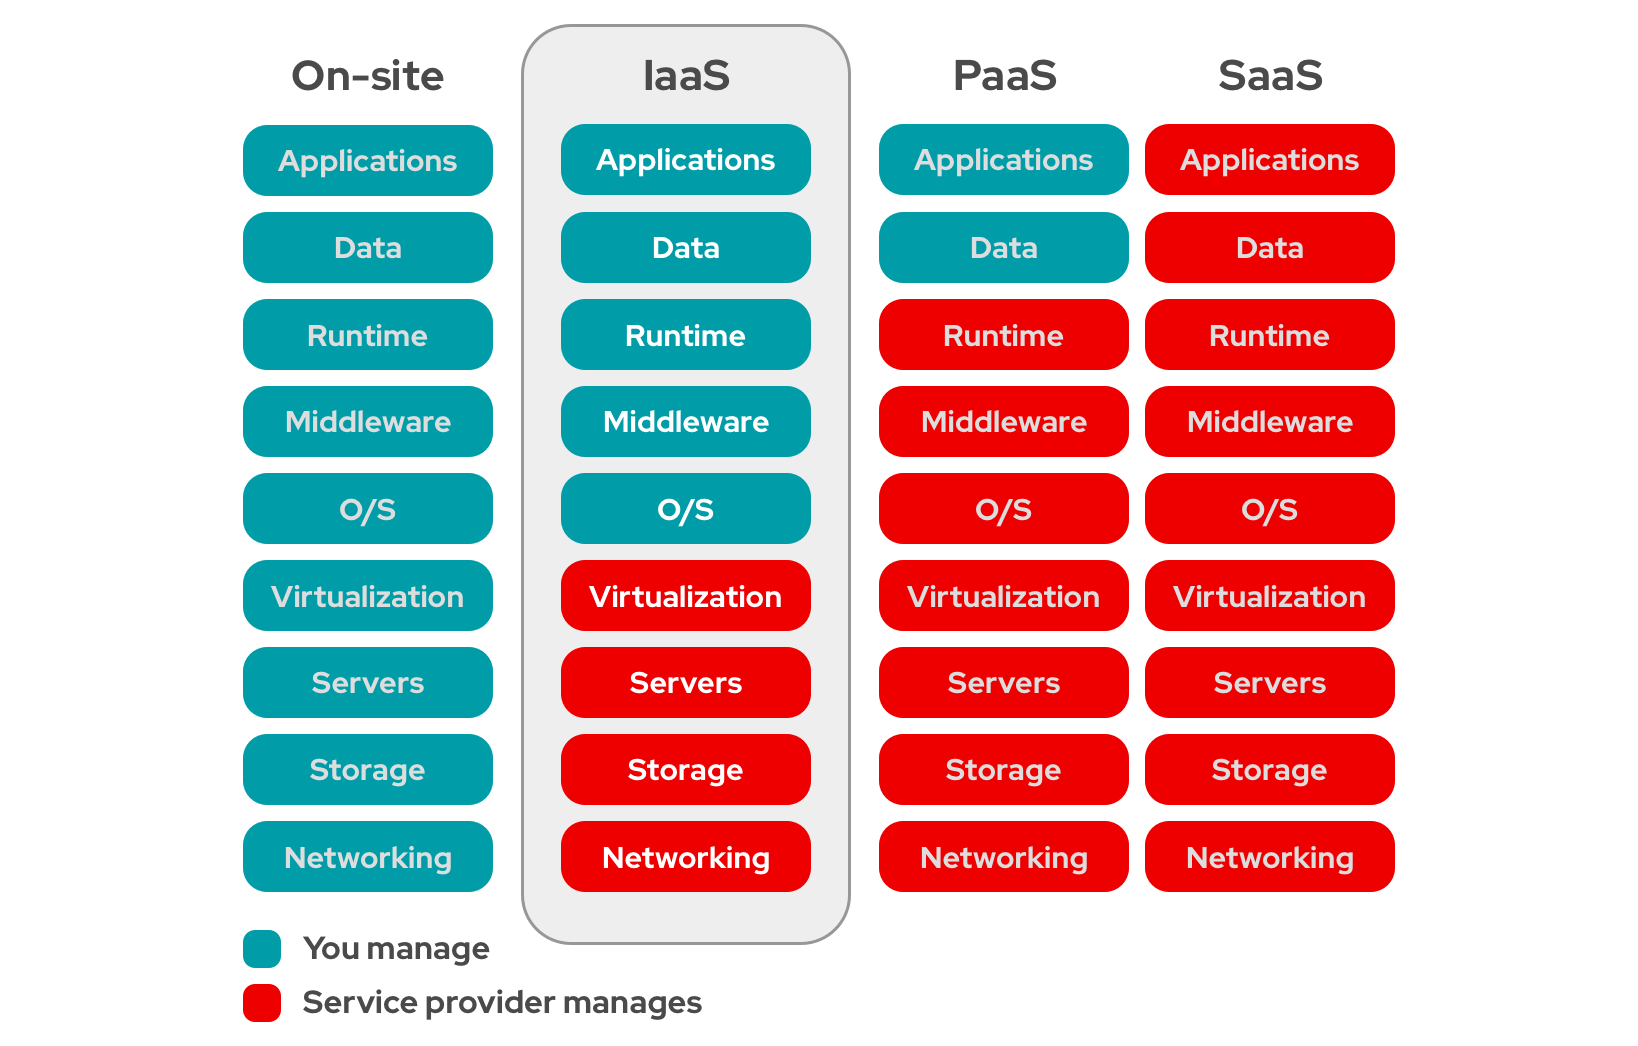
\includegraphics[scale=0.3]{as-a-Service_comparison.png}

\begin{center}
    \url{www.redhat.com/de/topics/cloud-computing/what-is-iaas}
\end{center}
"Most businesses use a combination of SaaS and IaaS cloud computing service models." \\
Also services like Security-as-a-Service (SaaS), Firewall-as-a-Service (FWaaS) or Software Infrastructure-as-a-Service (SIaaS) exist.

\section*{Cloud Providers} 
\textbf{Biggest Players} \hspace{11cm} \href{https://www.zdnet.com/article/the-top-cloud-providers-of-2021-aws-microsoft-azure-google-cloud-hybrid-saas/}{\textit{Source}}
\begin{enumerate}
    \item Amazon Web Services (AWS)
    \item Microsoft Azure
    \item Google Cloud and Anthos
    \item Alibaba Cloud (mainly China)
    \item IBM Cloud
    \item VMware (Dell)
\end{enumerate}
\textbf{Further Cloud Providers:}
\begin{itemize}
    \begin{multicols}{2}
        \item Salesforce (leading in SaaS)
        \item Oracle Cloud
        \item SAP Business Technology Platform (SAP BTP) \\
        (at least SAP HANA cloud is AWS)
        \item ServiceNow
        \item Microsoft Office 365
        \item OpenStack
        \item Kamatera
        \item Adobe (at least partially AWS!)
    \end{multicols}
\end{itemize}
\textbf{Cloud Services for Small Businesses:}
\begin{itemize}
    \begin{multicols}{2}
        \item Amazon S3
        \item Azure Storage
        \item Dropbox
        \item Openstack
        \item Office365 (One Drive, MS Teams)
        \item Google Drive
        \item iCloud
        \item Asana
        \item Shopify
        \item Slack
    \end{multicols}
\end{itemize}


\newpage
\section*{Misc}
\begin{itemize}
    \item Cloud-Enabler: primarily IT firms that develop hardware, software, storage, networking and other related products, serving as a cloud environment component.
    \item Cloud-Service-Provicer (CSP): vendors which provide Information Technology (IT) as a service over the Internet.
    \item Identify where a server is located: \url{https://research.domaintools.com/}
\end{itemize}


\subsection*{Researching \& ideas}
\begin{itemize}
    \item googleapi in content security policy $\rightarrow$ using google cloud services? \\
    $\Rightarrow$ No, googleapis aren't cloud services!
    
    How about learning something out of the CSP?
    
    \item DNS entries? DNS Resolver from AWS? or CloudFront servers? Amazon Route 53 (DNS Management Service)?
    
    \item Fiddler, Wireshark, analyzing traffic?

    \item cookies? (probably not?)
    
    \item Serialization objects? \\
    \url{view-source:https://www.dowjones.com/} contains \verb|amazon_s3_cache| element??
\end{itemize}


\subsection*{Websites}
\begin{itemize}
    \item \url{https://www.observa.com/} \\ 
    They get read-only access and scan your EC2 account via Nmap to detect if your database is publicly available, has open ports, ... 
    \item \url{https://www.shodan.io/} \\
    Search engine to find specific types of computers connected to the internet. Shows 10 results to user without an account and 50 to those with one. You can remove the restriction via a fee (university staff and students for free?).
\end{itemize}

\subsubsection*{Find out what websites are built with}
\begin{itemize}
    \item \url{https://builtwith.com}
    \item \url{https://www.wappalyzer.com/}
\end{itemize}


\newpage
\subsection*{Understanding AWS}
\begin{itemize}
    \item Identify if website uses AWS:
    
    "Amazon has 26 different web services. You can tell if the web server you are communicating with is hosted by Amazon EC2 by its IP address. You can't tell if there are EC2 instances behind a proxy you're talking to, though.

    You can tell if the domain name is resolved by an Amazon Route 53 DNS server.

    Besides that, you wouldn't really know what other services are being used unless they choose to make it obvious."
    
    \item EC2:
    
    Elastic Compute Cloud, IaaS (and SaaS); provides scalable computing capacity in the Amazon Web Services (AWS) Cloud
    
    \item S3:
    
    Simple Storage Service; really good for static websites (html, css, js) but doesn't support server-side scripting languages (php,...)
    
    You can easily host a website via S3 bucket options. If you want your own domain name you have to register it and use Route 53: on resolution there are awsdns entries (e.g. ns-183.awsdns-22.com. / s3-website)
    
    \item AWS Certificate Manager is a private CA service.
    
    \item AWS Direct Connect \\
    "If you want a setup without using the internet at all, that's when you look at AWS Direct Connect" 
    
    Internal network is linked to an AWS Direct Connect location over Ethernet (one end on personal router, the other one to an AWS Direct Connect router). ISPs are bypassed
    
    
    
\end{itemize}

\subsection*{Understanding Azure / Office365}
Services in more than 600 services. Besides typical IaaS, SaaS and PaaS also Blockchain Workbench, CDN, IoT,... They are categorized into 5 core services:
\begin{itemize}
    \item Application Services (AI, Analytics, IoT, ...)
    \item Data Services (Storage, SQL DB, Cache,...)
    \item Development Services (Development tools, ...)
    \item Compute Services (VMs, Container Service,...)
    \item Network Services (CDN, DNS,...)
\end{itemize}
To privately connect to Azure, Expressroute is being used (AWS: Direct Connect) connections that don't go over the public internet. \\ 
If access to email sent from those domains, headers will contain wealth of information (\verb|Received-header, X-header|). 



\newpage
\section*{How to identify used Cloud Services}
\subsection*{Information "provided" by the company}
\begin{itemize}
    \item \textbf{DNS Entries}
    \begin{itemize}
        \item \textbf{Nameserver}\\
        For (some?) cloud services:
    
        \verb|dig @8.8.8.8 +trace website.com|
        
        When inspecting the trace there can be found different cloud nameserver, indicating that the website is set up / uses the listed cloud services. \\
        \textit{So far: AWS ("awsdns"), Azure ("azure-dns"), Google cloud ("ns-cloud-c2.googledomains.com", Cloudflare ("ns.cloudflare")}
        
        Attention: e.g. SAP uses AWS services, however resolving their DNS entry does not show it. This is because their webpage doesn't use AWS services directly.
        
        \item \textbf{MX-record} \\
        Can show e.g. usage of Office365
        \begin{verbatim}
nslookup
set q=MX
ais-security.de
        \end{verbatim}
        
        \item \textbf{TXT-record}
        
        \verb|dig txt website.com|
        \begin{itemize}
            \item \verb|MS=ms| is for Office365
            \item \verb|ZOOM_verify_<hash>| is for Zoom
            \item \verb|include:spf.protection.outlook.com| is for outlook
            \item \verb|dropbox-domain-verification| is for Dropbox
            \item \verb|google-site-verification=<hahs>| is for GCP (Google Workspace)
        \end{itemize}
        
        
        \item \url{https://dnsdumpster.com/}
        
    \end{itemize}
    
    \item \textbf{Certificates}
    \begin{itemize}
        \item AWS: 
    
        has own "Certificate Managers" (ACM) ("Amazon Root CA 1", "Amazon", "aws.amazon.com") the later partially issuing websites hosted on AWS
        
        \item Google: 
    
        has own Certificate Authority called "Certificate Authority Service" 
        
        \item Cloudflare: 
    
        own CA e.g. \verb|Cloudflare Inc ECC CA-3| issuing coinbase.com
    \end{itemize}
    
    \item \textbf{JavaScript}

    By inspecting \verb|view-source|, JavaScript from used cloudproviders can be found
    \begin{itemize}
        \item AWS: \verb|aws.amazon.com|, \verb|s3.amazonaws.com| %pfizer.com
        \item (Cloudflare:
        \verb|cdnjs.cloudflare.com| \textit{unsure: some say cdn is cloud service, others say not}, \verb|cloudflare|.) \\
        $\rightarrow$ not a cloud service we were looking for!
        \item Microsoft: \verb|office.com|, \verb|azureedge|, \verb|voracio|
    \end{itemize}
    
    Unclear: Is there really a cloud service in use or simply cdn-service? 
    
    
    \item \textbf{Response Headers}
    
    \verb|server| attribute can reveal information 
    \begin{itemize}
        \item \textbf{Amazon server:} \verb|AmazonS3|, \verb|ECS|, 
        \item \textbf{Azure server:} \verb|Windows-Azure-Web|, \verb|Microsoft-Azure-Application*| \\
        Furthermore, Azure hosted websites mostly have attributes like \verb|x-azure-ref|, \verb|x-azure-ref-originshield| \\
        Often times \verb|Microsoft-IIS/10.0| servers are used, but this doesn't always implies  that Azure is used.
        %\item \textbf{Cloudflare server:}
        %\verb|cloudflare|
    \end{itemize}
    
    
    \item \textbf{IP address}
    
    To get the IP address simply run \verb|dig DOMAIN +short| \\
    Afterwards, run \verb|whois IP_address| 
    
    \textit{It states that the site is behind e.g. Cloudflare. But does it always means that the company who is running the server (e.g. cloudflare) is also a cloud provider for the website?}
    
    
    \item \textbf{Autonomous Systems}
    
    Lookup of used AS: \url{https://hackertarget.com/as-ip-lookup/}
    
    List of all AS's: \url{https://bit.ly/34lCIMz}, \url{https://www.ripe.net/}
    
    See which domains are hosted by a specific AS: \url{https://ipinfo.io/AS16509#domains}
        
    See the IP's for an ASN: \url{https://mxtoolbox.com/asn.aspx}
    
	\textbf{ASNs reserved for Azure}
    \begin{itemize}
        \item Public ASNs: 8074 (ripe states ASNumber: 8068-8075), 8075 , 12076 (for ExpressRoute peering)
        \item Private ASNs: 65515, 65517, 65518, 65519, 65520
    \end{itemize}    
    
    \newpage
    \textbf{Amazon's ASN's used (partially) for AWS services} \\ \\
    \begin{tabular}[h]{| c | p{3cm} | p{2.5cm} | p{5cm} |}
        \hline
        \textbf{ASN} & \textbf{Region} & \textbf{for VPN connections} & \textbf{Remarks} \\ \hline
        AS7224 & - & - & \href{https://search.arin.net/rdap/?query=AS7224}{used for AWS} \\ \hline
        AS14618 & - & - & \href{https://search.arin.net/rdap/?query=AS14618}{used for AWS} \\ \hline
        AS16509 & - & - & \href{https://search.arin.net/rdap/?query=AS16509}{used for AWS (S3)} \\ \hline
        AS17493 & Asia Pacific Singapore Region & \checkmark & \href{https://stat.ripe.net/app/launchpad/S1_17493_C13C31C4C34C9C22C28C20C15C6C7C14C26C29C30C17C2C21C33C16C10}{used for AWS} \\ \hline
        AS10124 & Asia Pacific Tokyo region & \checkmark & there are no domains hosted on this ASN, it also has no neighbours \\ \hline
        AS9059 & for Europe & \checkmark & there are no domains hosted on this ASN, it also has no neighbours \\ \hline
        AS7224 & for all other regions & \checkmark &  \\ \hline
        AS58588 &  &  & \href{https://stat.ripe.net/app/launchpad/S1_58588_C13C31C4C34C9C22C28C20C15C6C7C14C26C29C30C17C2C21C33C16C10}{actually out of service} \\ \hline
        64512 - 65534 &  &  & Private ASNs \\ \hline
        %AMAZON ASNs which aren't used for AWS services
        %\item AS8987  Amazon Data Services Ireland Ltd; has nothing to do with AWS
        %\item AS38895 AMAZON-AS-AP Amazon.com Tech Telecom; has nothing to do with AWS
        %\item AS39111 ADSI-AS Amazon EU DC AS; has nothing to do with AWS
    \end{tabular}
   
    Why is there an overlap on the private ASNs from AWS and Azure?
    
    
    \item \textbf{Zoom}
    
    Zoom has 4 different subscription options (\textit{Basic, Pro, Business, Enterprise}). When subscripted to \textit{Business} or \textit{Enterprise}, the company gets an own domainname (\verb|companyname.zoom.us|).
    
    \begin{itemize}
        \item \textbf{Identify Business and Enterprise model:} 
        \begin{itemize}
            \item Check if \verb|website.zoom.us| or \verb|website-TLD.zoom.us| exists.
            \item Create a 'DB' collecting all subdomains of \verb|.zoom.us| and check if company is included.\\
            \url{https://searchdns.netcraft.com/} or \url{https://pentest-tools.com/information-gathering/find-subdomains-of-domain} for even more subdomains (nearly all when doing a "Full Scan"?; output can be saved in PDF)
            \item To prove that you own the domain, one of three verification methods have to be made:
            \begin{itemize}
                \item txt-Record: \verb|ZOOM_verify_<hash>| token
                \item HTML file on the domain
                \item meta-tag on domain's homepage
            \end{itemize}
        \end{itemize}
    \end{itemize}
    
    
    \item \textbf{MS-Teams}
    
    %MS Teams has 3 main subscription options (\textit{Free, Business Basic, Business Standard}).
    
    \href{https://support.microsoft.com/en-us/office/find-your-friends-and-family-in-teams-711bfcef-9e40-49d5-8df7-ee071a048c91#ID0EACAAA=Desktop}{"To find someone in Teams:"}
    \begin{enumerate}
        \item Click Search from the top of the main Teams window.
        \item In the Search for people and chats field, search for a contact by their Phone, Email, or Name.
    \end{enumerate}
    Note: users may opt out of search
    
    
    \item \textbf{Dropbox}
    
    Subscription options for teams: \textit{Standard}, \textit{Advanced}, and \textit{Enterprise}.
    
    \begin{itemize}
        \item Using \textit{Advanced}, \textit{Enterprise}, \textit{Education} or \textit{Professional} subscription, you can see when someone (full name and email address) has viewed a file if she has read-access. Furthermore you can see if they are the member of a business-team (and the corresponding name) or not. \\
        \textbf{Idea} / Untypical way: create a Dropbox account (cheapest in this case probably \textit{Professional}) and create a file which is then being shared with the company. See if they accessed via "Guest" or with an Dropbox account. \\
        \textbf{Problem}: costs money; isn't a clear indicator whether they really (don't) use Dropbox because they might access as guest even though they have an account; they might not access at all; however, this has to be practically proofed
        
        \item Business-Teams and Enterprise subscription models offer "domain analysis" \textit{(seeing the usage of private Dropbox accounts)} and "account registration". To be able to use this feature, you have to proof that you control the domain:
        \begin{itemize}
            \item TXT Record: \verb|dropbox-domain-verification|
            \item HTML file
            \item meta-tag on homepage
        \end{itemize}
    \end{itemize}
    
    
    \item \textbf{Salesforce}
    
    (SaaS specialized in customer relationship management)
    
    \begin{itemize}
        \item Salesforce services are embedded into a website. Therefore, searching / crawling a website for \verb|"salesforce"| might give an indication. \\
        $\rightarrow$ \href{https://www.wappalyzer.com/lists/?technologies=salesforce}{Wappalyzer}
        
        \item Connection Finder: \\
        Available in \textit{Group}, \textit{Professional}, \textit{Enterprise}, and \textit{Unlimited Editions} you can find out if your partners are Salesforce customer (if they enabled Connection finder).
    \end{itemize}
    
    
    \item \textbf{VMWare}
    
    Related to the \href{https://thehackernews.com/2021/06/alert-critical-rce-bug-in-vmware.html?m=1}{\textit{RCE bug in VMWare vCenter Server}}, we can identify the servers via \href{https://www.shodan.io/search?query=vCenter+Server}{\textit{shodan.io}} and even more specifically with the search query \\ \verb|product:"VMware vCenter Server"|.
    
    %Their cloud computing virtualization platform is called vSphere

 
\end{itemize}

\subsection*{Information gained on unintended ways}
\begin{itemize}
    \item 
\end{itemize}


\newpage
\section*{How to not identify used Cloud Services}
\begin{itemize}
    \item Dedicated Cloud Connectivity: \\ AWS Direct Connect / Azure Expressroute / GCP Dedicated Interconnect: they run over Ethernet so traffic can only be observed by physically attaching a device to the network
\end{itemize}


\end{document}
